% -*- root: main.tex -*-
%-------------------------------------------------------------------------------
\chapterimage{chapter_head_3.pdf} 

%-------------------------------------------------------------------------------
\chapter{ROS 설치 (SBC or VirtualBox)}\label{cha:ros_install_sbc}

%-------------------------------------------------------------------------------
\section{가상 머신에 ROS Indigo 설치하기}\index{가상 머신에 ROS Indigo 설치하기}

%-------------------------------------------------------------------------------
\subsection{우분투 14.04 이미지 준비}\index{우분투 14.04 이미지 준비}

ROS의 사용은 기본적으로 \textbf{섹션~\ref{sec:ROSInstallation}~\nameref{sec:ROSInstallation}(pp.\pageref{sec:ROSInstallation})} 에서와 같이 우분투를 기본 운영체제로 사용한다. 그 이외에도 윈도우즈와 OS X 등에서도 사용은 가능하나 일부 기능을 사용 못하거나 일일이 소스를 받아서 재컴파일할 필요가 있다. 그래서 이번 챕터에서는 윈도우즈에 가상 머신을 설치하여 윈도우즈 환경에서 우분투를 실행하는 가상 머신을 활용하는 방법에 대해서 다룰 예정이다. 간단히 테스트하거나 튜토리얼 정도는 이 방법으로 할 수 있을 것이다. 참고로 가상 머신은 본 챕터에서 소개하는 오픈소스 기반의 VirtualBox\footnote{\url{https://www.virtualbox.org/}} 이외에도 상용 제품인 VMware\footnote{\url{http://www.vmware.com/}}, Parallels\footnote{\url{http://www.parallels.com/}} 등이 있다. 자신에게 맞는 것을 사용하도록 하자.

이 방법은 가상 머신 사용으로 인해 2개의 운영체제가 CPU를 나누어 쓰게되어 속도면에서 매우 본래 목적인 ROS 사용에 있어서 속도면에서 지장을 준다. 필자는 가상 머신보다는 우분투만 사용하거나 혹은 윈도우즈와 멀티부팅으로 사용하기를 추천한다. 간단한 테스트 목적 및 학습 목적이라면 이 방법으로 \textbf{챕터~\ref{cha:RosPrograming}~\nameref{cha:RosPrograming}(pp.\pageref{cha:RosPrograming})} 수행에는 전혀 문제 없다.

우선, 그림\ref{fig:download_ubuntu}와 같이 \url{http://www.ubuntu.com/download/desktop/} 에서 우분투 ISO 이미지파일을 다운로드 하자. 우분투는 14.04.x LTS 로 선택하고, 자신의 컴퓨터의 사양에 따라 32bit 혹은 64bit 를 골라 다운로드 하자.

\begin{figure}[h]
\centering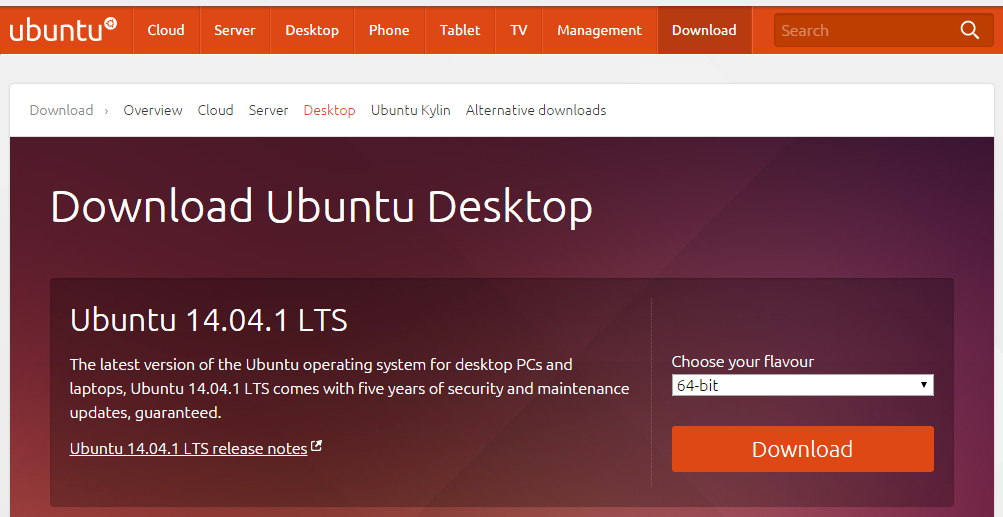
\includegraphics[width=0.5\columnwidth]{pictures/chapter3/ubuntu_web.png}
\caption{우분투 이미지 파일 다운로드}
\label{fig:download_ubuntu}
\end{figure}

%-------------------------------------------------------------------------------
\subsection{Virtualbox 설치}\index{Virtualbox 설치}

\begin{figure}[h]
\centering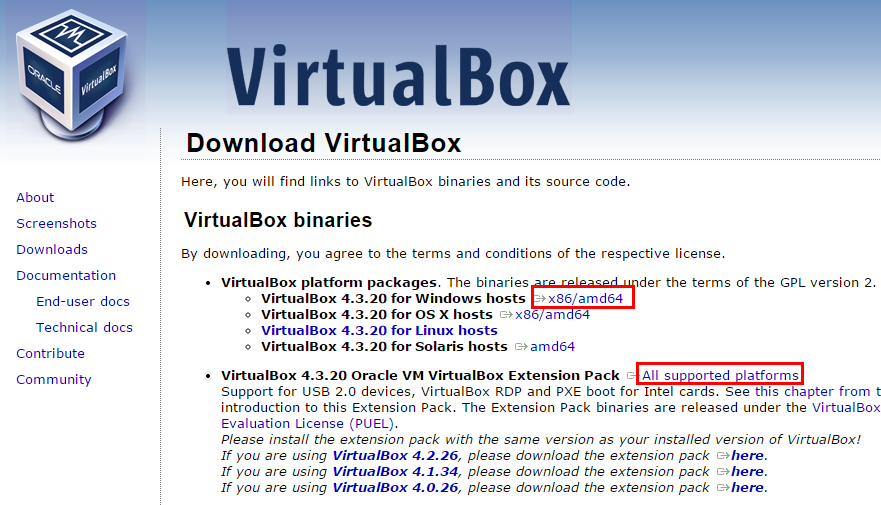
\includegraphics[width=0.7\columnwidth]{pictures/chapter3/virtual_box_web.png}
\caption{Virtual Box 다운로드}
\label{fig:download_vm}
\end{figure}

그림\ref{fig:download_vm}와 같이 VirtualBox 4.3.xx for Windows hosts 와 VirtualBox 4.3.20 Oracle VM VirtualBox Extension Pack 을 다운로드 하자. 설치 방법은 매우 간단하다. 다음의 설치 과정의 그림들을 참고해 가며 설치하도록 하자.

\begin{figure}[h]
\centering
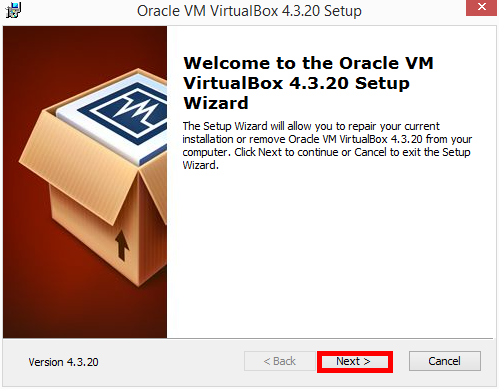
\includegraphics[width=0.42\columnwidth]{pictures/chapter3/vm1.png}
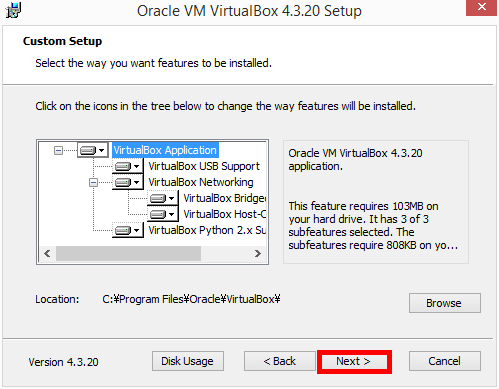
\includegraphics[width=0.42\columnwidth]{pictures/chapter3/vm2.png}
\end{figure}

\begin{figure}[h]
\centering
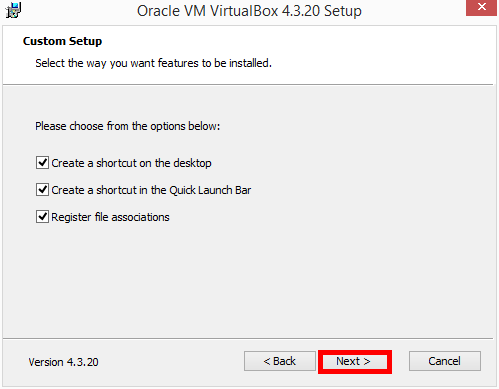
\includegraphics[width=0.42\columnwidth]{pictures/chapter3/vm3.png}
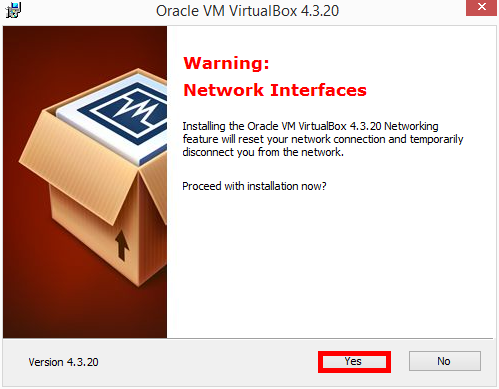
\includegraphics[width=0.42\columnwidth]{pictures/chapter3/vm4.png}
\end{figure}

\newpage

\begin{figure}[h]
\centering
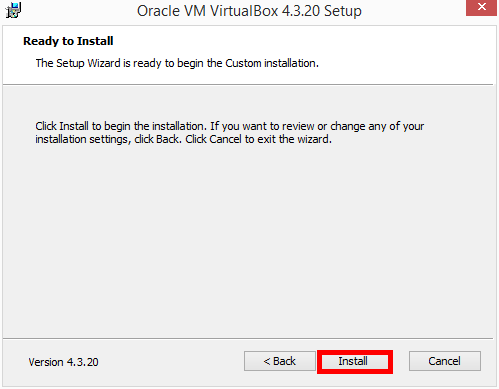
\includegraphics[width=0.49\columnwidth]{pictures/chapter3/vm5.png}
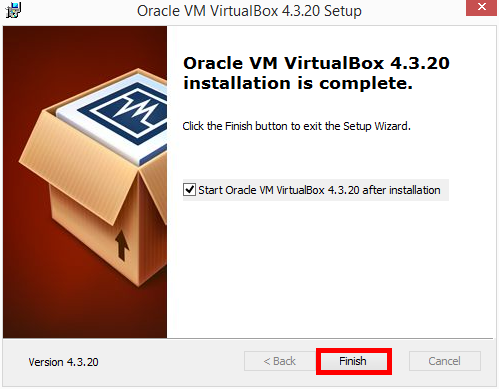
\includegraphics[width=0.49\columnwidth]{pictures/chapter3/vm6.png}
\end{figure}

\begin{figure}[h]
\centering
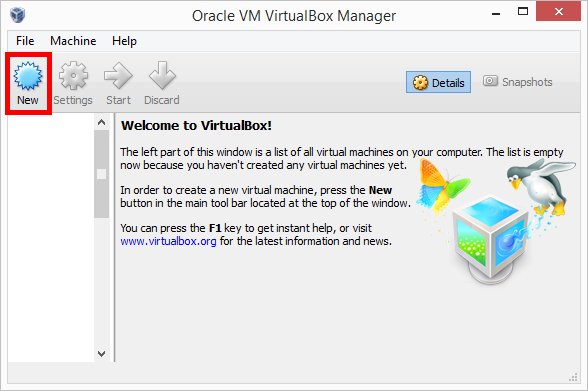
\includegraphics[width=0.49\columnwidth]{pictures/chapter3/vm7.png}
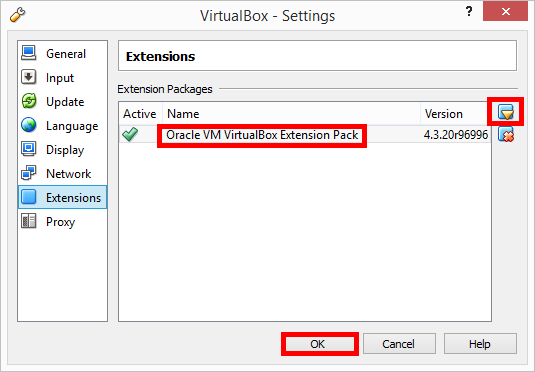
\includegraphics[width=0.49\columnwidth]{pictures/chapter3/vm8.png}
\end{figure}

\begin{figure}[h]
\centering
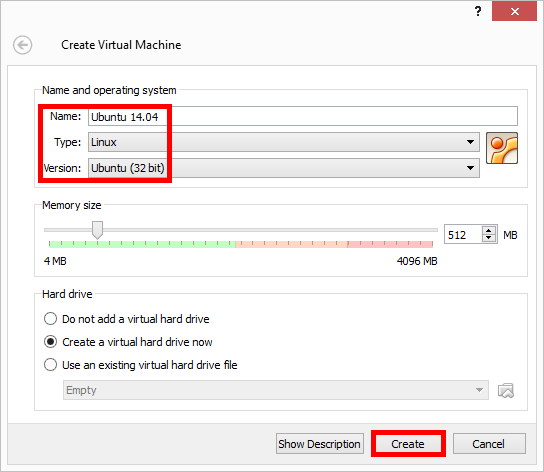
\includegraphics[width=0.49\columnwidth]{pictures/chapter3/vm9.png}
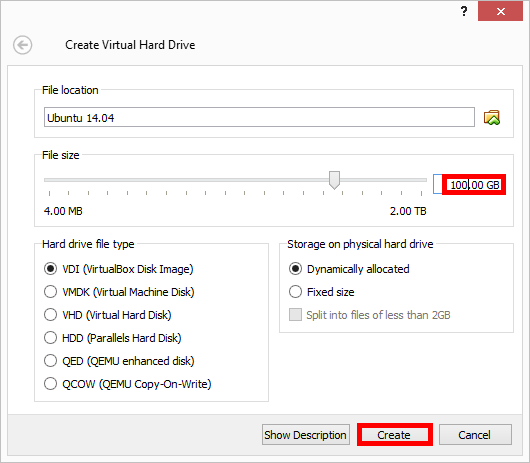
\includegraphics[width=0.49\columnwidth]{pictures/chapter3/vm10.png}
\end{figure}

\newpage

\begin{figure}[h]
\centering
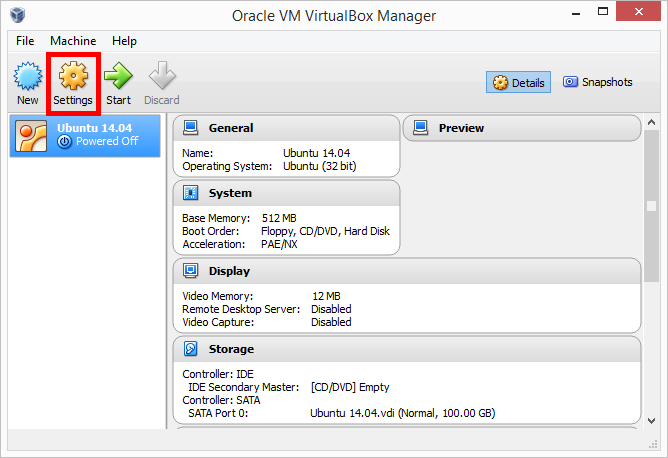
\includegraphics[width=0.49\columnwidth]{pictures/chapter3/vm11.png}
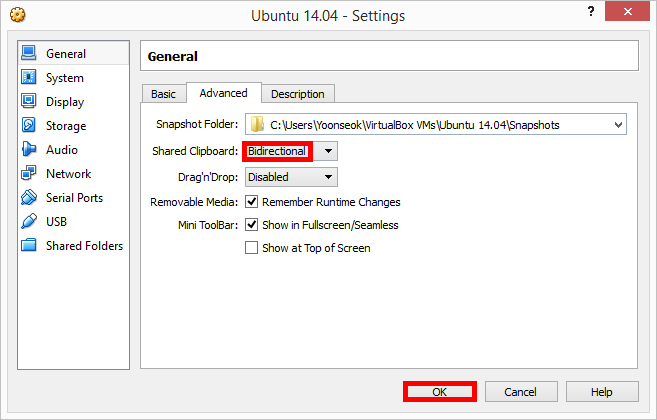
\includegraphics[width=0.49\columnwidth]{pictures/chapter3/vm12.png}
\end{figure}

\begin{figure}[h]
\centering
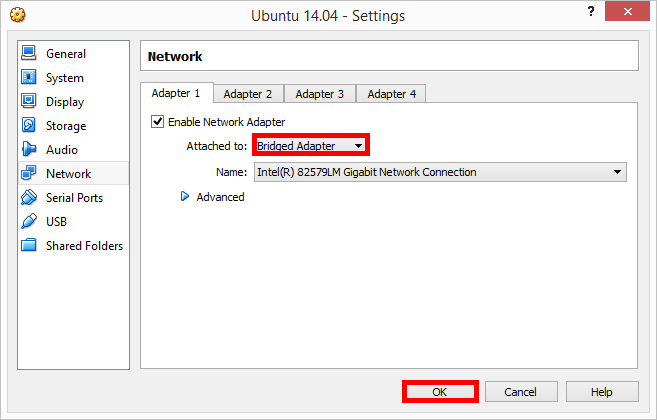
\includegraphics[width=0.49\columnwidth]{pictures/chapter3/vm13.png}
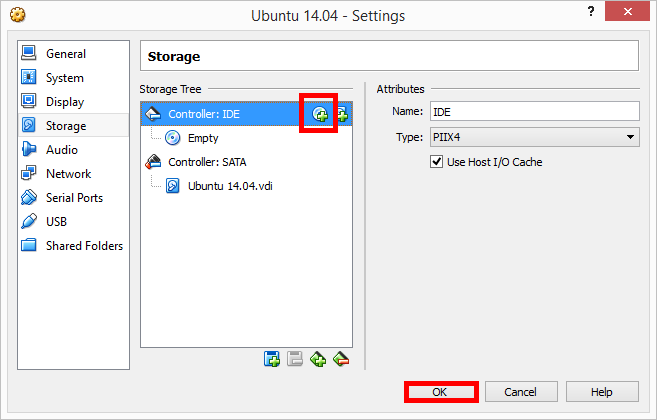
\includegraphics[width=0.49\columnwidth]{pictures/chapter3/vm14.png}
\end{figure}

\begin{figure}[h]
\centering
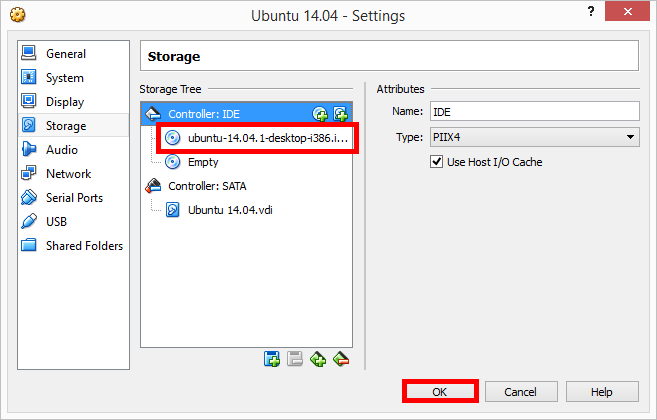
\includegraphics[width=0.49\columnwidth]{pictures/chapter3/vm15.png}
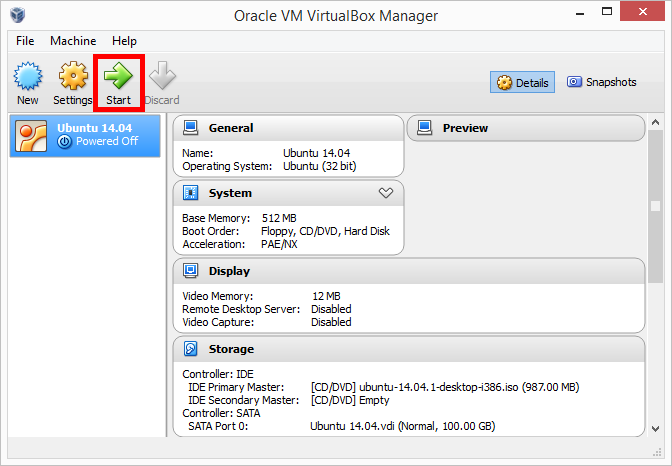
\includegraphics[width=0.49\columnwidth]{pictures/chapter3/vm16.png}
\end{figure}

\newpage

\noindent
다음 그림들을 참고해가며 우분투를 설치하도록 하자. 우분투 설치가 마무리 되면 우분투 배포판이 나온 이후의 갱신에 대해서 다음의 명령어로 업데이트와 업그레이드를 해주도록 하자.

\vspace{\baselineskip}
\begin{lstlisting}[language=ROS]
$ sudo apt-get update && sudo apt-get upgrade
\end{lstlisting}

\begin{figure}[h]
\centering
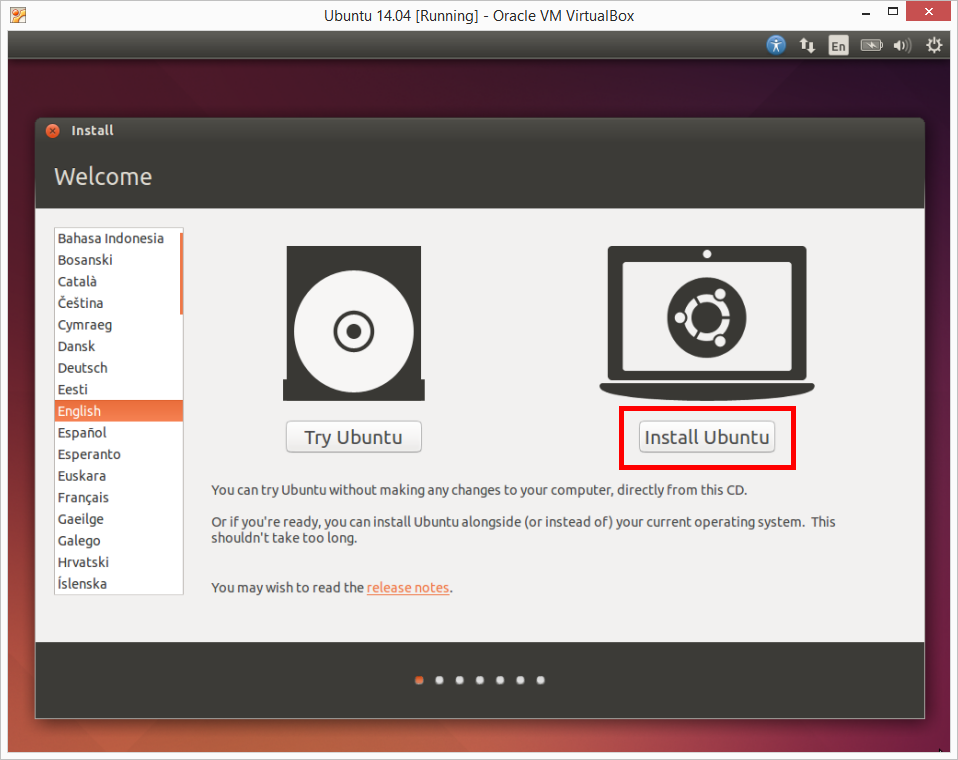
\includegraphics[width=0.45\columnwidth]{pictures/chapter3/vm17.png}
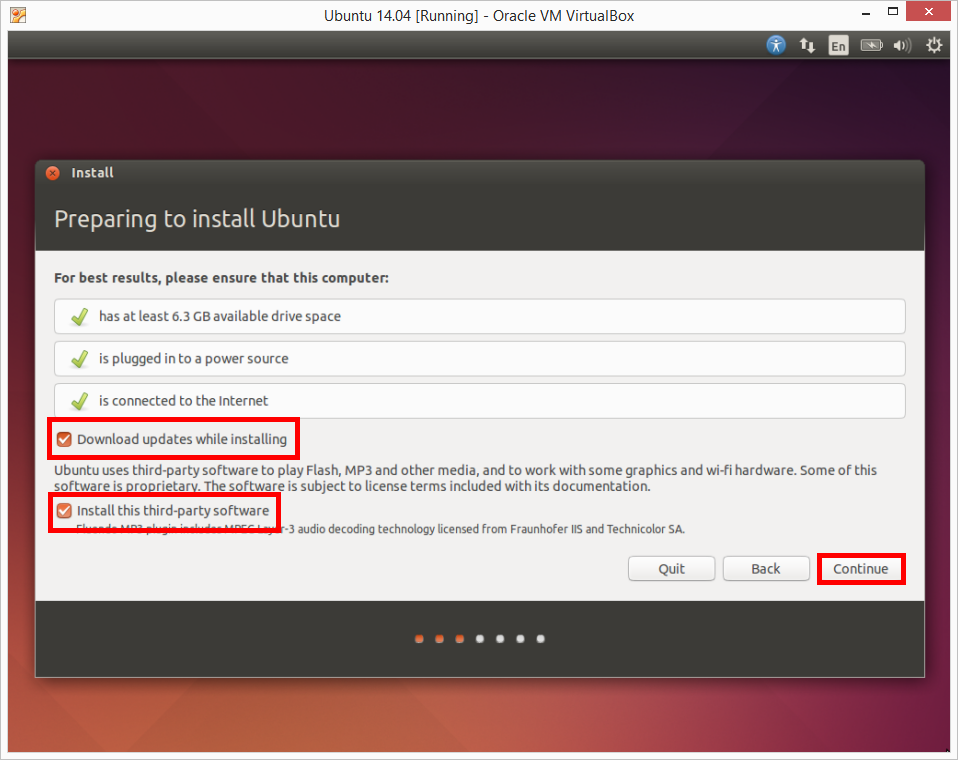
\includegraphics[width=0.45\columnwidth]{pictures/chapter3/vm18.png}
\end{figure}

\begin{figure}[h]
\centering
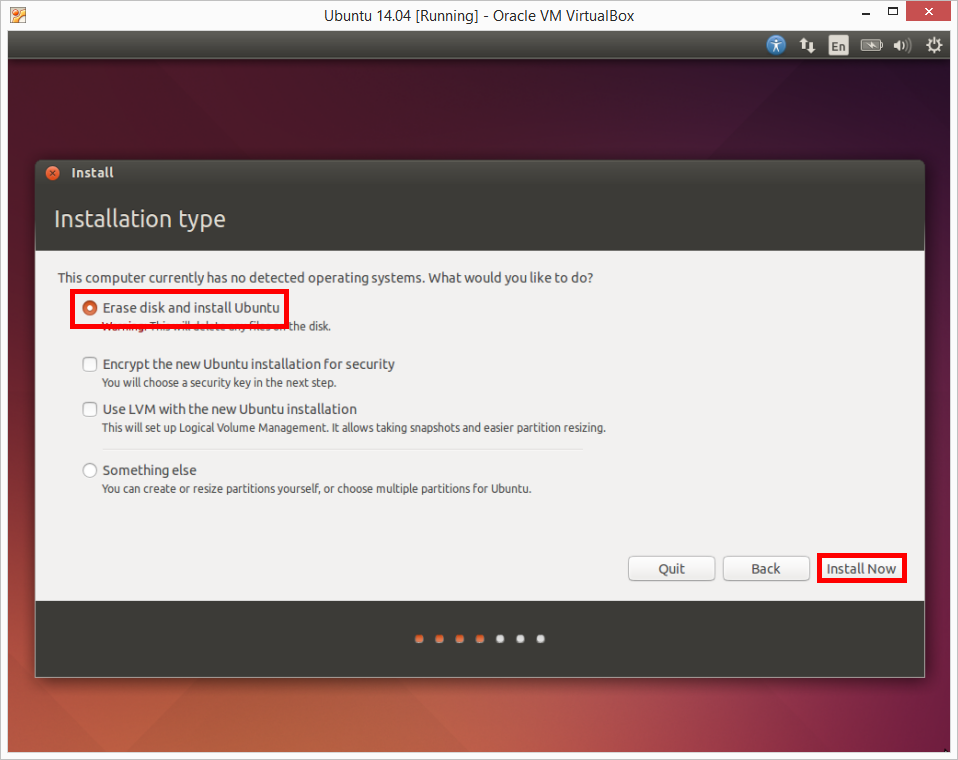
\includegraphics[width=0.45\columnwidth]{pictures/chapter3/vm19.png}
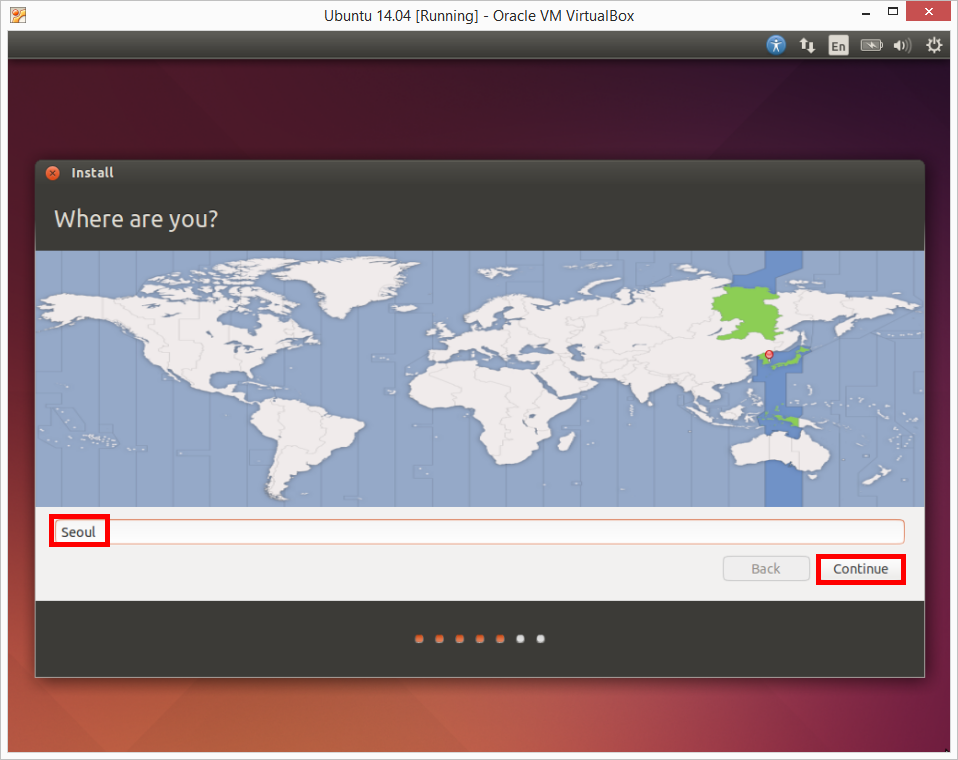
\includegraphics[width=0.45\columnwidth]{pictures/chapter3/vm20.png}
\end{figure}

\begin{figure}[h]
\centering
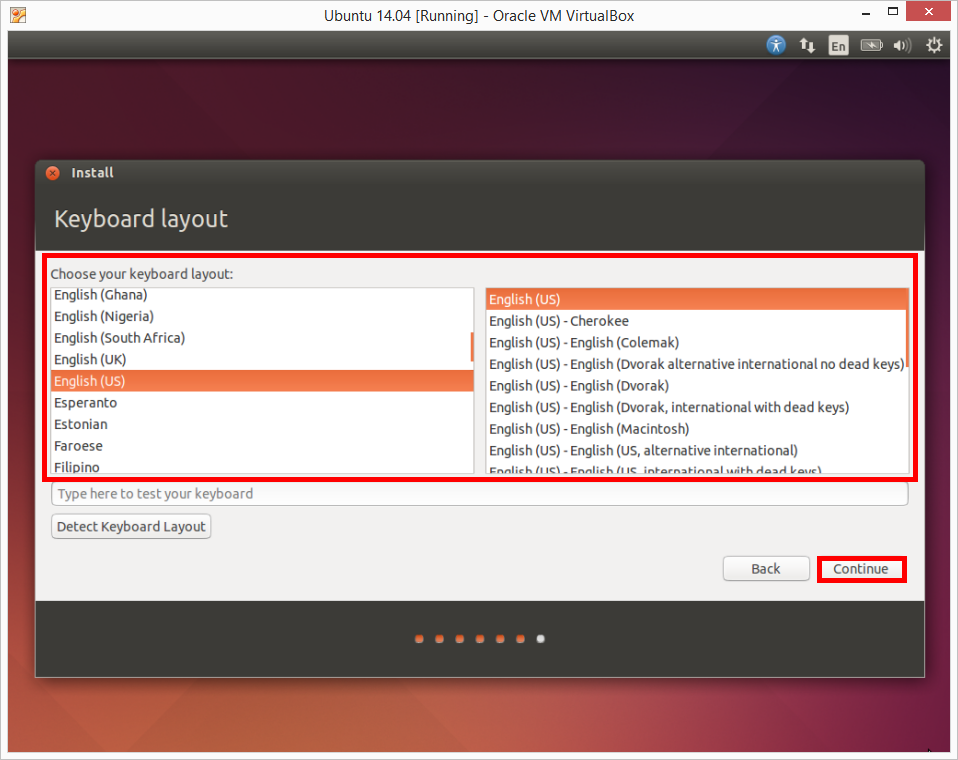
\includegraphics[width=0.45\columnwidth]{pictures/chapter3/vm21.png}
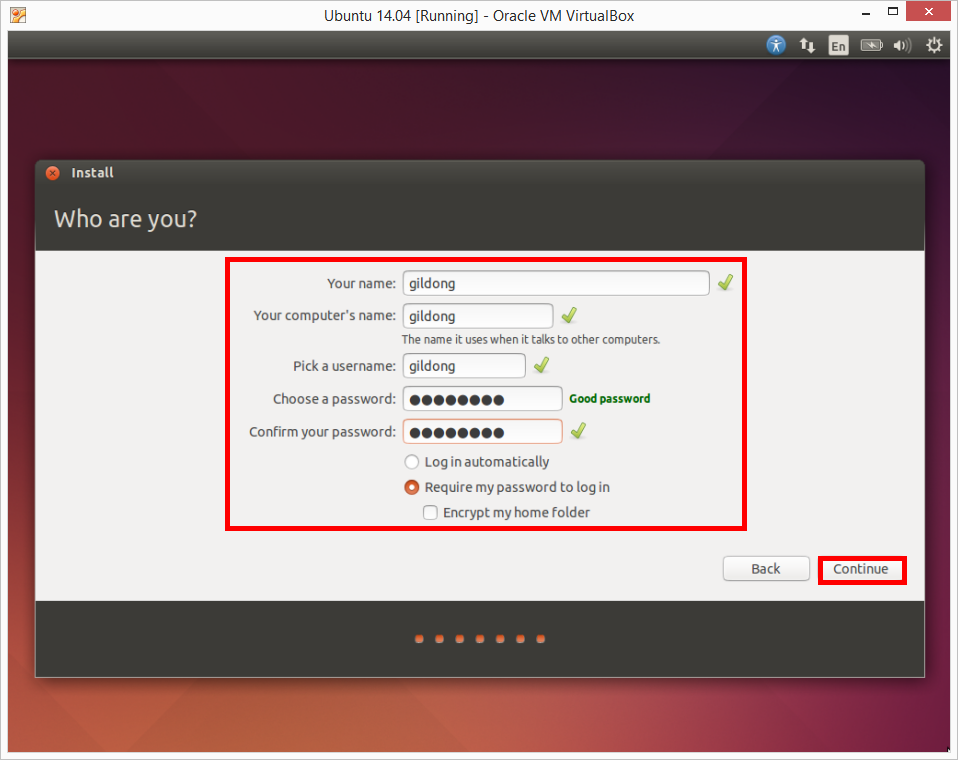
\includegraphics[width=0.45\columnwidth]{pictures/chapter3/vm22.png}
\end{figure}

\newpage

\begin{figure}[h]
\centering
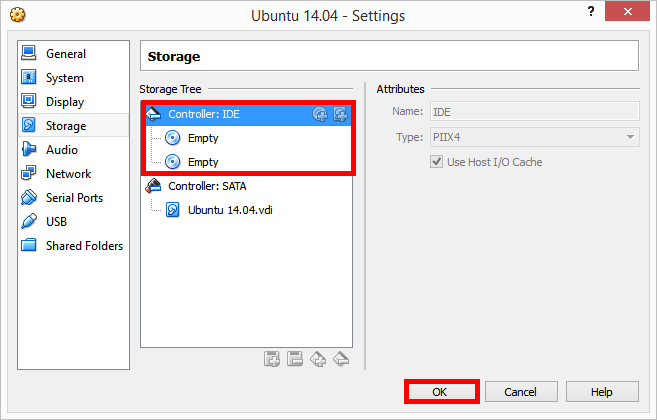
\includegraphics[width=0.49\columnwidth]{pictures/chapter3/vm23.png}
\end{figure}

%-------------------------------------------------------------------------------
\subsection{ROS Indigo 설치하기}\index{ROS Indigo 설치하기}

ROS Indigo 설치는 \textbf{섹션~\ref{sec:SimpleInstallation}}에서 설명한 간단 설치 방법으로 설치하도록 하겠다. 터미널 창을 열고 (Ctrl + Alt + t) 다음과 같이 간단 설치용 스크립트를 다운로드 한 후, 스크립트를 실행하여 ROS Indigo 설치하도록 하자.

\vspace{\baselineskip}
\begin{lstlisting}[language=ROS]
$ wget https://raw.githubusercontent.com/oroca/oroca-ros-pkg/master/ros_indigo_install.sh
$ sh ros_indigo_install.sh
\end{lstlisting}

\noindent
이제 모든 설치 작업이 완료되었다. 제대로 설치가 됐는지 알아보기 위하여 다음과 같이 roscore를 실행, 그리고 또 다른 새로운 터미널 창을 열고 turtlesim\_node를 구동하면 그림와 같이 실행될 것이다. 이 거북이를 보게 된다면 성공적으로 설치가 완료된 것이다. 추가적인 개발 환경 설정은 \textbf{섹션~\ref{subsec:envrionment}~\nameref{subsec:envrionment}(pp.\pageref{subsec:envrionment})}을 참고하도록 하자.

\vspace{\baselineskip}
\begin{lstlisting}[language=ROS]
$ roscore
$ rosrun turtlesim turtlesim_node
\end{lstlisting}

\begin{figure}[h]
\centering
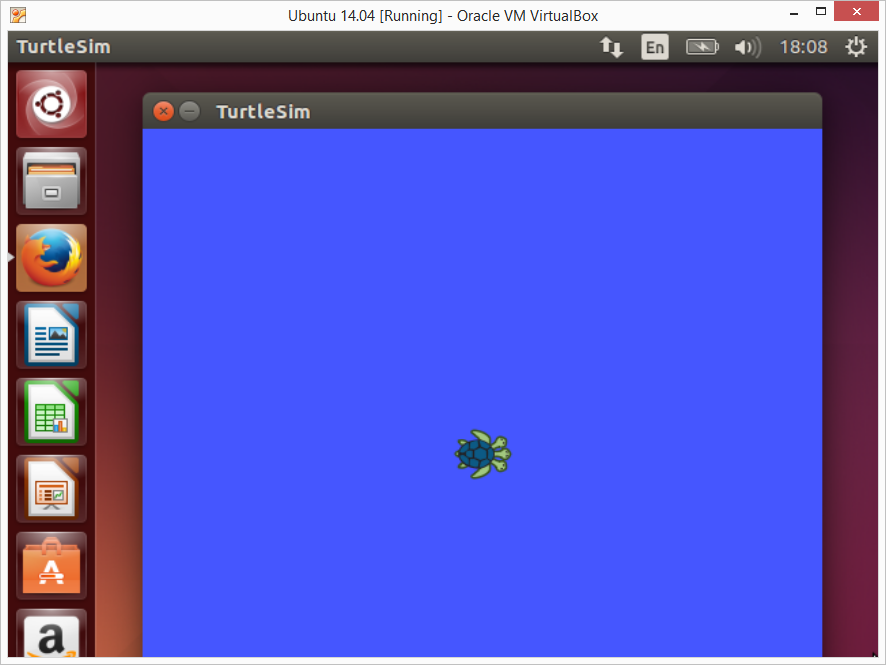
\includegraphics[width=0.6\columnwidth]{pictures/chapter3/vm24.png}
\end{figure}

%-------------------------------------------------------------------------------
\newpage
\section{라즈베리파이에 ROS Indigo 설치하기}\index{라즈베리파이에 ROS Indigo 설치하기}

라즈베리파이(Raspberry Pi\footnote{\url{http://www.raspberrypi.org/}})는 영국의 라즈베리파이재단\footnote{\url{http://www.raspberrypi.org/education-fund/}}에서 아이들의 컴퓨터 교육을 위해 개발한 싱글보드컴퓨터(SBC, Single Board Computer)이다. 그러한 이유에서, 가격도 거의 최저 마진에 가깝다. 모델 A의 경우 25달러, 모델 B의 경우 35달러에 판매되고 있다. 이는 라즈베리파이 재단 총감독인 에벤 업튼(Eben Upton)이 어린이들의 교과서 가격에 맞추어 가격을 책정했기 때문이라고 한다. 필자가 처음 컴퓨터를 접했을 때는 인텔 486 컴퓨터 및 초창기 펜티엄으로, CPU는 133MHz~300MHz 에 가격은 대략 250만원에 상당했다. 그 시절과 비교하면 대략 두 배의 성능의 CPU성능에 크기는 신용카드의 크기로 축소되었고 가격은 4만원 정도로 1/60로 떨어졌다. 

또한, C언어, 자바, 파이썬, 루비 등의 프로그래밍 언어뿐만 아니라, 어린이용 GUI방식의 스크래치(Scratch) 프로그래밍도 사용할 수 있도록 되어있다. 더욱이 매력적인 것은 데스크톱에서 찾아 볼 수 없는 범용 입출력 포트인 GPIO 를 제공하고 있어서 전자 공작 및 로봇 제어 등의 학습에도 이용 가능하게 되어있다는 것이다. 다른 싱글보드컴퓨터와는 달리 에벤 업튼이 꿈꾸는 컴퓨터의 보급 및 어린이들의 교육에 매우 적절한 제품이 아닐까 싶다. 또한 라즈베리파이는 단순한 보드에 그치지 않고, 많은 유저들의 참여로 웹 서버, 데이터베이스, 파일서버, 미디어 센터, 게임기 등의 다양한 프로젝트가 진행 중이며, 최근에는 GPIO를 이용한 전자공작 교육 및 로봇 제어 등에도 사용되고 있다\cite{lp2013raspberry}.

이 만큼 라즈베리파이는 그 활용도가 높은데 오늘은 로봇쪽으로 활용하기 위해 ROS 설치법에 대해 알아보도록 하자. 우선 ROS 를 설치하기 전에 라즈페리파이의 공식 OS인 데비안 데비안 계열의 Raspbian\footnote{\url{http://www.raspbian.org/}}을 설치하도록 하자. 라즈베리파이 공식 웹페이지(\url{http://www.raspberrypi.org/downloads/})에 접속하여 RASPBIAN 최신판을 다운로드 하자.

\begin{figure}[h]
\centering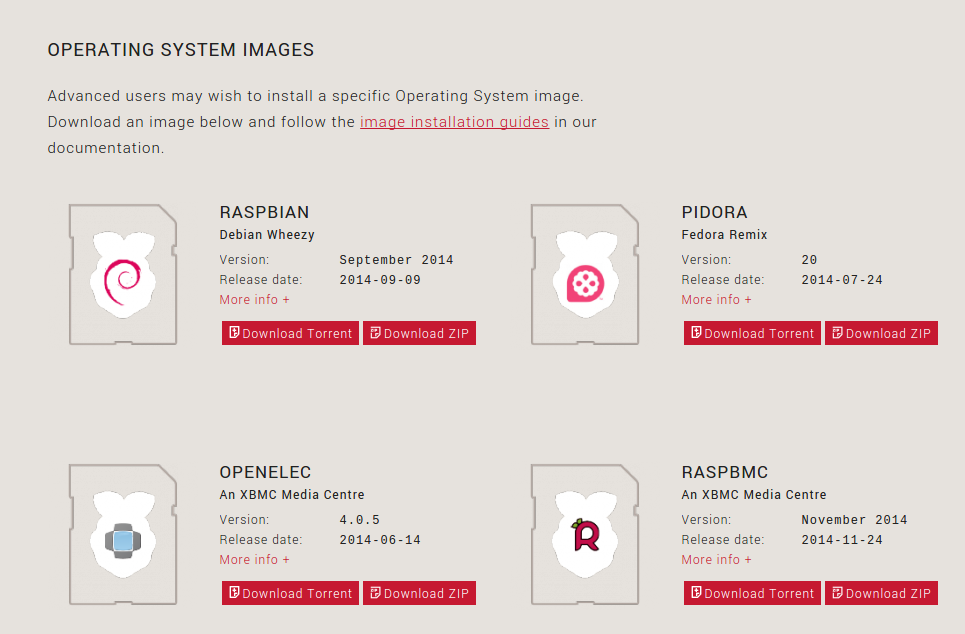
\includegraphics[width=\columnwidth]{pictures/chapter3/raspberrypi_raspbian_download.png}
\caption{라즈베리파이의 다양한 OS 지원}
\end{figure}

\newpage

\noindent
다운로드가 완료되면 터미널 창을 열어 다음과 같이 압축 해제를 해주어 이미지 파일을 얻도록 하자.

\vspace{\baselineskip}
\begin{lstlisting}[language=ROS]
$ unzip  2014-09-09-wheezy-raspbian.zip
\end{lstlisting}

\noindent
압축 해제한 이미지 파일을 SD 카드에 넣도록 하자. 완전 포맷되지 않은 SD 카드의 경우, 기존 파티션을 삭제 하도록 하자. 파티션 수정을 위하여 GUI를 지원하는 disks를 이용할 것이다. 터미널 창에서 gnome-disks 를 실행하자. 그 뒤 디스크 목록에서 해당 SD 카드를 선택하면 기존에 사용했던 SD 카드라면 그림\ref{fig:partition_init1} 좌측과 같이 기존 파티션들이 보일 것이다. 그 하단의 \textbf{-} 버튼을 클릭하여 기존 파티션을 모두 삭제하여 모든 영역을 Free Space로 만들면 그림\ref{fig:partition_init1} 우측과 같은 결과를 얻을 수 있다.

\vspace{\baselineskip}
\begin{lstlisting}[language=ROS]
$ gnome-disks
\end{lstlisting}

\begin{figure}[h]
\centering
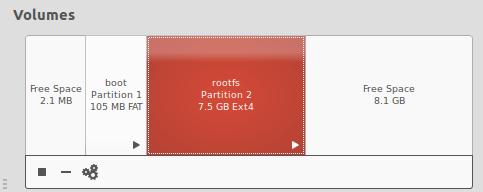
\includegraphics[width=0.49\columnwidth]{pictures/chapter3/odroid_partition1.png}
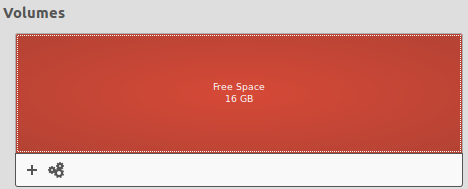
\includegraphics[width=0.48\columnwidth]{pictures/chapter3/odroid_partition2.png}
\caption{기존 파티션(좌)과 파티션 초기화(우)}
\label{fig:partition_init1}
\end{figure}

\noindent
그 다음 그림\ref{fig:raspbian_partition} 좌측의 disks 화면의 우측 상단의 버튼을 클릭하여 Restore disk image... 을 실행하자. 그림\ref{fig:raspbian_partition}의 추측 그림처럼 imgae to Restore 의 파일 선택에서 이전 압축 해제한 이미지 파일을 선택하고 Start Restoring 를 클릭하면 라즈비안 이미지가 리스토어 되게 된다. 리스토어가 완료되면 그림\ref{fig:raspbian_partition_new} 과 같이 새로운 파티션들이 생성 되었음을 확인할 수 있다.

\vspace{\baselineskip}
\begin{figure}[h]
\centering
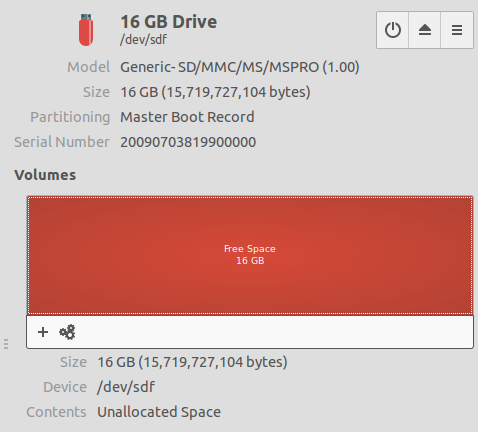
\includegraphics[width=0.4\columnwidth]{pictures/chapter3/odroid_sd.png}
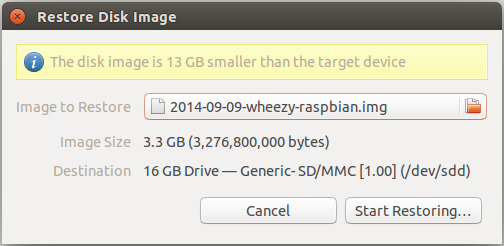
\includegraphics[width=0.5\columnwidth]{pictures/chapter3/raspberrypi_disks2.png}
\caption{디스크가 초기화된 상태(좌), 리스토어 준비 과정(우)}
\label{fig:raspbian_partition}
\end{figure}

\begin{figure}[h]
\centering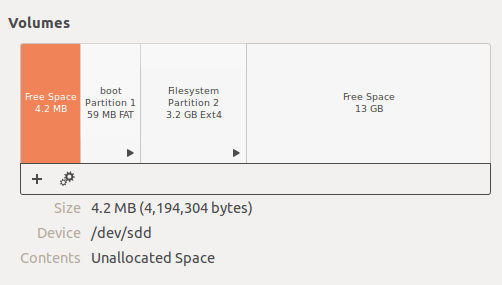
\includegraphics[width=0.6\columnwidth]{pictures/chapter3/raspberrypi_disks3.png}
\caption{새롭게 구성된 파티션}
\label{fig:raspbian_partition_new}
\end{figure}

\newpage

\begin{exercise}[SD 카드에 이미지 파일 넣는 다른 방법]
disks 이외에도 dd bs=4M if=2014-09-09-wheezy-raspbian.img of=/dev/sdd 처럼 dd 명령어를 이용하는 방법이 있으며, 윈도우즈의 경우 Win32DiskImage\footnote{\url{http://sourceforge.net/projects/win32diskimager/}}를 이용하여 손쉽게 이미지 파이을 SD카드에 넣을 수 있다.
\end{exercise}

\vspace{\baselineskip}
라즈베리파이 이미지 파일이 들어있는 SD 카드를 라즈베리파이에 삽입한 후, 전원을 넣고 부팅되면 그림\ref{fig:raspberrypi_raspbian_on}와 같이 라즈비안이 실행된다. 참고로 초기 로그인시 아이디는 \textbf{pi} 이며 패스워드는 \textbf{raspberry}이다. 나중에 직접 패스워드를 변경 해주도록 하자.

\begin{figure}[h]
\centering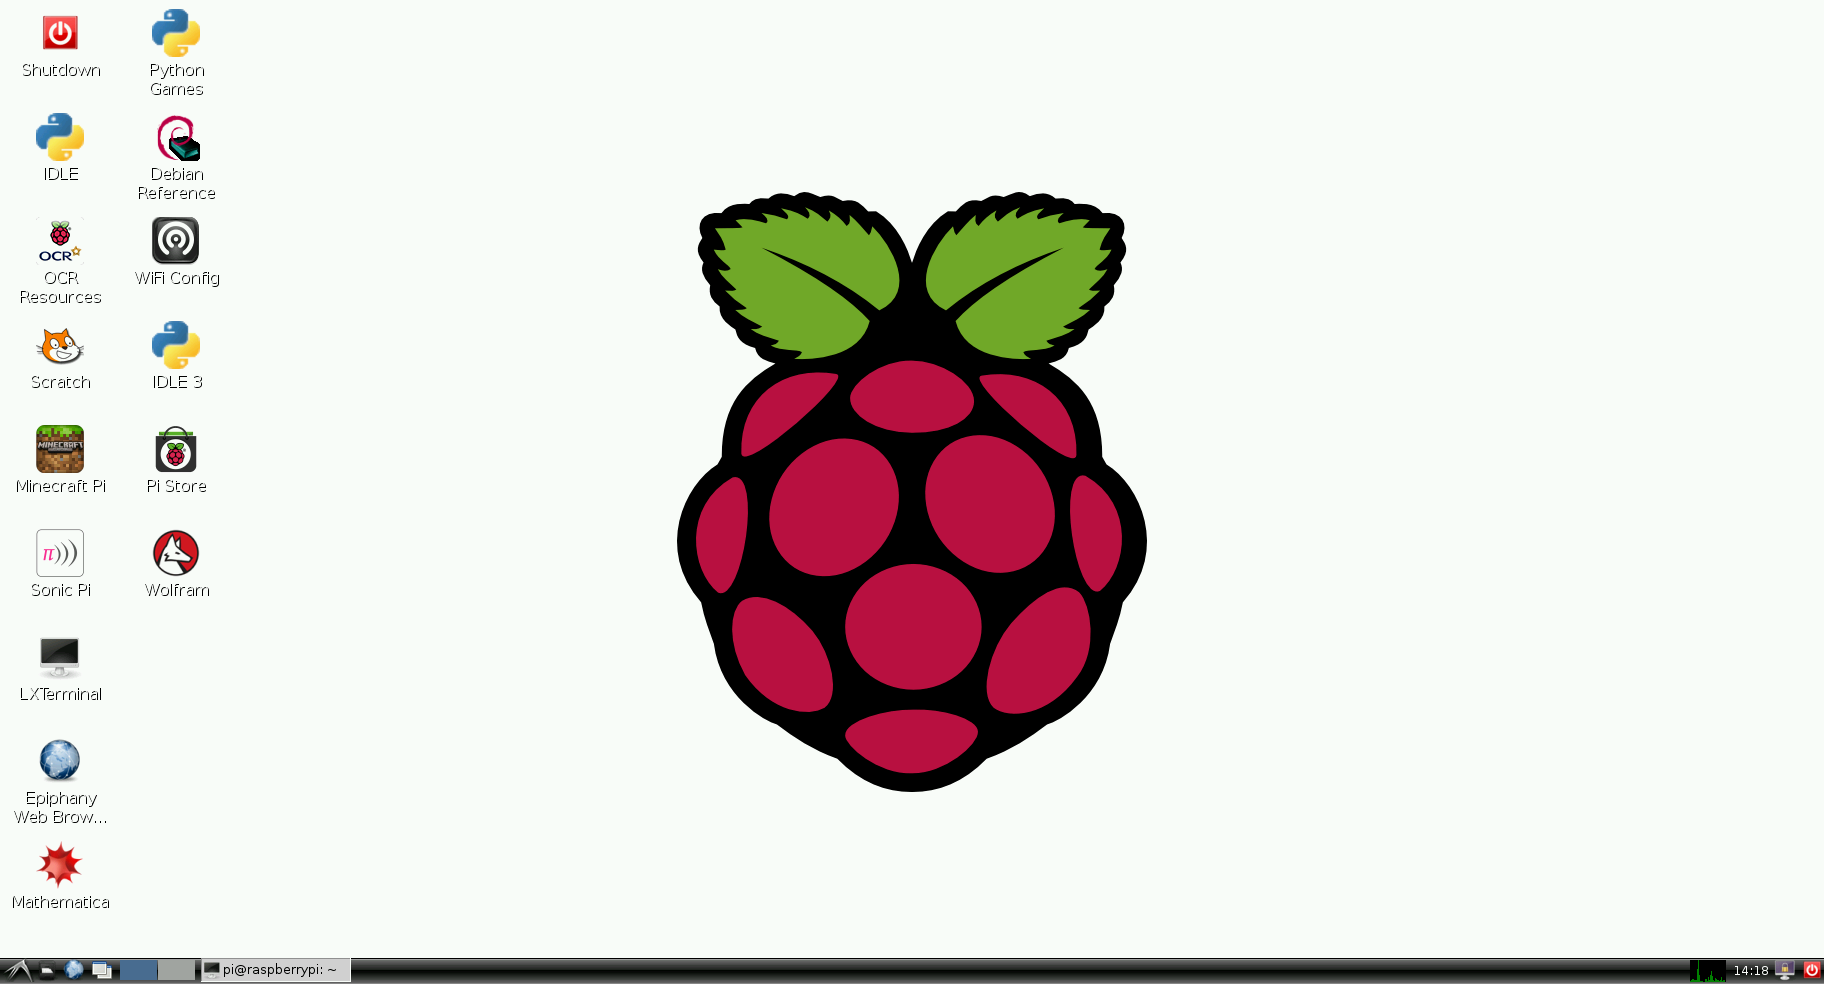
\includegraphics[width=0.9\columnwidth]{pictures/chapter3/raspberrypi_raspbian_desktop.png}
\caption{라즈비안의 데스트콥 화면}
\label{fig:raspberrypi_raspbian_on}
\end{figure}

우선, 현재 SD 메모리의 일부 부분만 사용할 수 있도록 되어 있기 때문에 메모리를 리사이즈 할 필요가 있다. 기본 탑재 터미널인 lxterminal을 실행하여 다음과 같이 라즈비안 설정을 실행하자. 그 후 그림\ref{fig:raspberrypi_expand_filesystem1}와 같이 메모리 리사이즈를 하기 위하여 1. Expand Filesystem 를 선택하여 리사이징을 해주자.

\vspace{\baselineskip}
\begin{lstlisting}[language=ROS]
$ sudo raspi-config
\end{lstlisting}

\begin{figure}[h]
\centering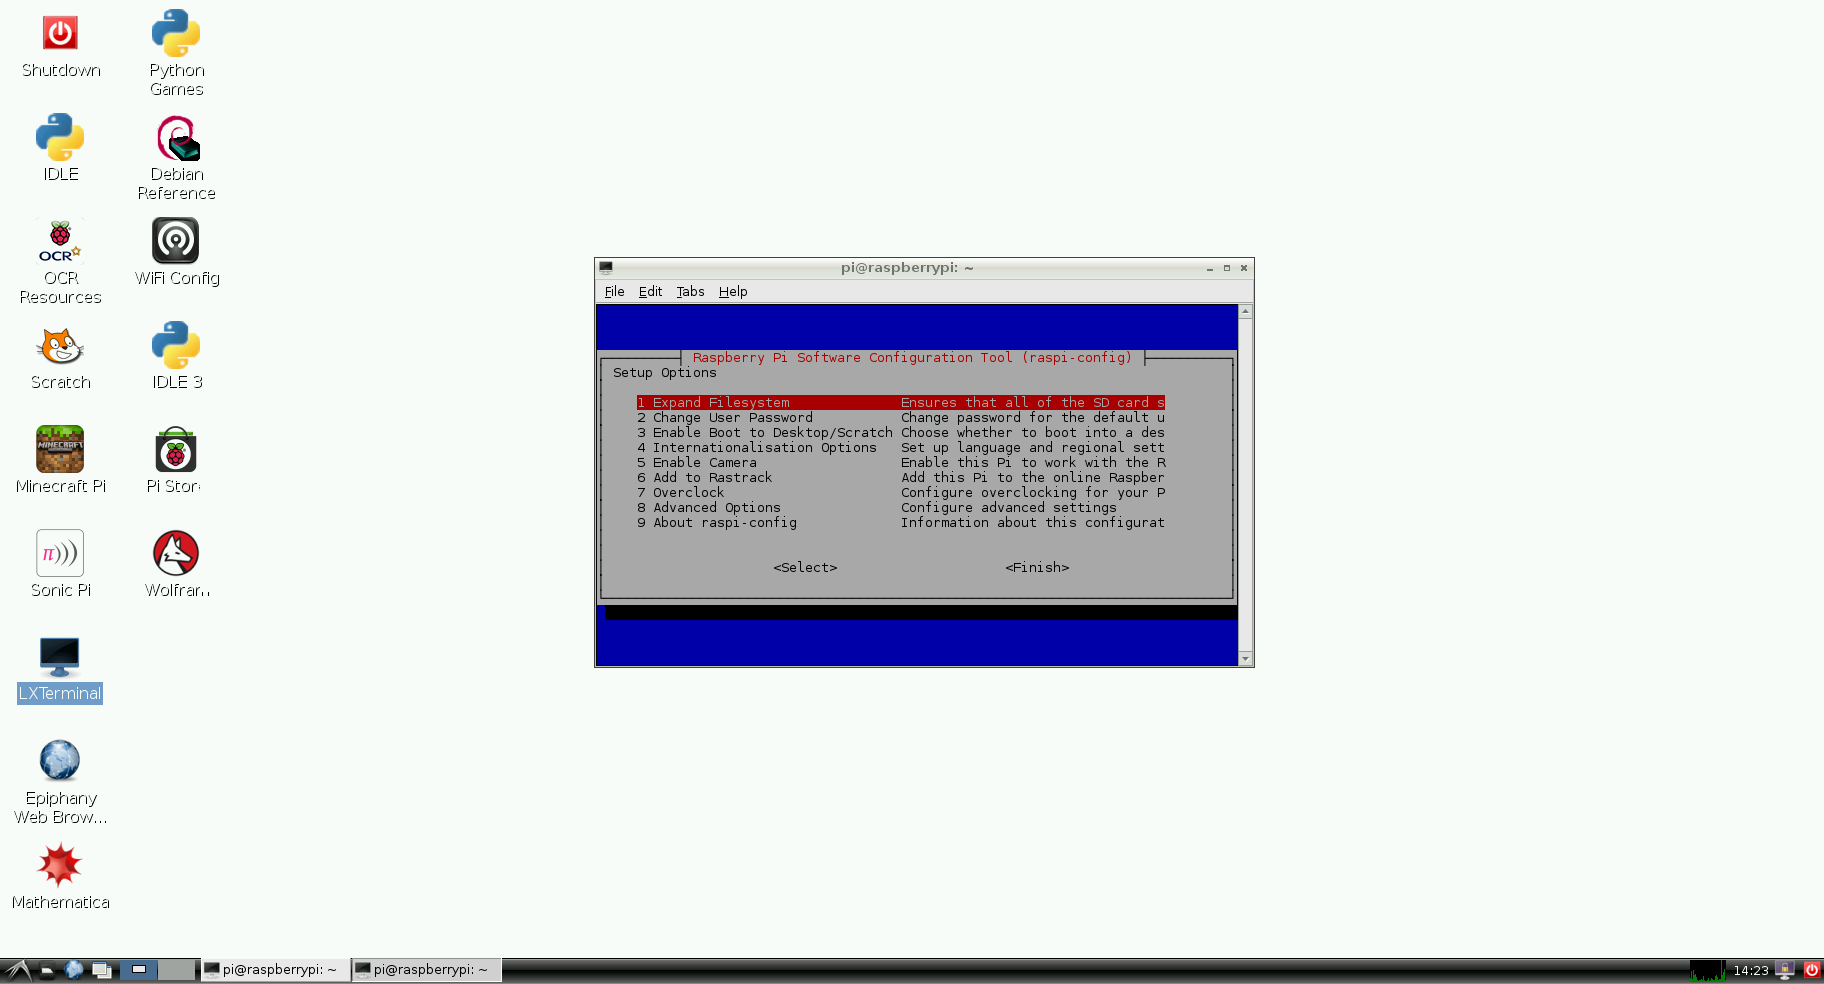
\includegraphics[width=0.7\columnwidth]{pictures/chapter3/raspberrypi_expand_filesystem1.png}
\caption{라즈비안 설정}
\label{fig:raspberrypi_expand_filesystem1}
\end{figure}

\begin{figure}[h]
\centering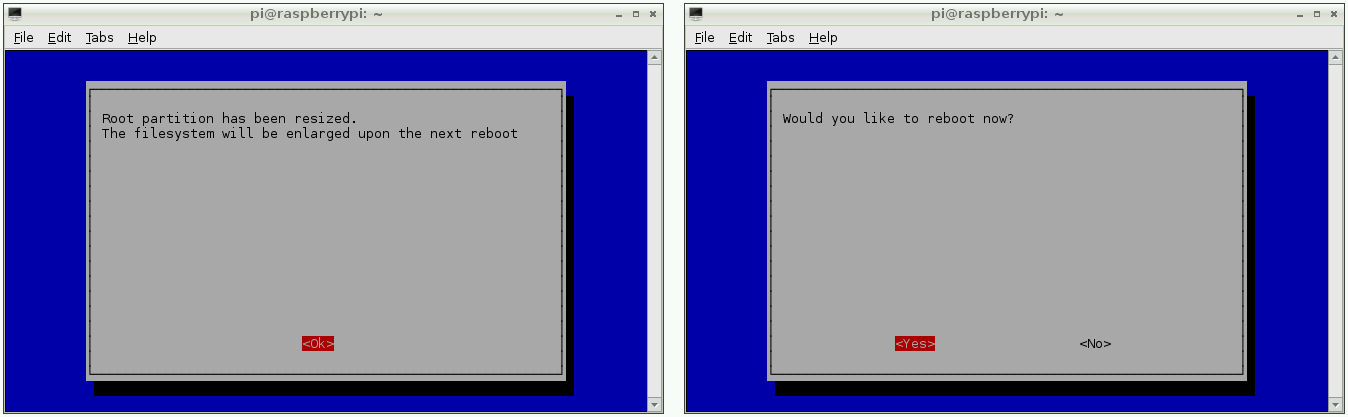
\includegraphics[width=\columnwidth]{pictures/chapter3/raspberrypi_expand_filesystem2.png}
\caption{SD 메모리의 리사이징}
\label{fig:raspberrypi_expand_filesystem2}
\end{figure}

리사이징이 완료되었으며 아래와 같이 재부팅이 되고 다시 라즈비안 데스크톱이 실행되면 다음의 명령어로 ROS Indigo\footnote{\url{http://wiki.ros.org/ROSberryPi/}}를 시작해보자.

\begin{lstlisting}[language=ROS]
$ sudo sh -c 'echo "deb http://packages.ros.org/ros/ubuntu wheezy main" > /etc/apt/sources.list.d/ros-latest.list'
$ wget https://raw.githubusercontent.com/ros/rosdistro/master/ros.key -O - | sudo apt-key add -
$ sudo apt-get update
$ sudo apt-get upgrade
$ sudo apt-get install python-setuptools
$ sudo easy_install pip
$ sudo pip install -U rosdep rosinstall_generator wstool rosinstall
$ sudo rosdep init
$ rosdep update
\end{lstlisting}

다음에는 다음과 같이 catkin work space 폴더를 만들고 catkin\_make 가 정상 작동하는지 확인해야 하는 것이 기본적인 ROS 설치 방법이나 라즈비안의 경우 catkin\_make가 바이너리 파일로 제공되지 않는다. 다음과 같은 순서로 catkin\_make 를 설치하도록 하자. 이 과정에는 의존관계에 있어서 libconsole\_bridg 및 Liblz4-dev 설치 과정이 포함되어 있다. 이는 대략 2시간이 소요된다.

\begin{lstlisting}[language=ROS]
$ source /opt/ros/indigo/setup.bash
$ mkdir -p ~/catkin_ws/src
$ cd ~/catkin_ws/src
$ rosinstall_generator ros_comm --rosdistro indigo --deps --wet-only --exclude roslisp --tar > indigo-ros_comm-wet.rosinstall
$ wstool init -j8 src indigo-ros_comm-wet.rosinstall
$ mkdir ~/ros_catkin_ws/external_src
$ sudo apt-get install checkinstall cmake
$ cd ~/ros_catkin_ws/external_src
$ sudo apt-get install libboost-system-dev libboost-thread-dev
$ git clone https://github.com/ros/console_bridge.git
$ cd console_bridge
$ cmake .
$ sudo checkinstall make install
\end{lstlisting}

checkinstall이 실행되고 EOF 구문에서 엔터키를 누르고, 2번째 항목에 console\_bridg 라 적혀있는 부분을 libconsole\_bridg 으로 변경하자.

\begin{lstlisting}[language=ROS]
$ cd ~/ros_catkin_ws/external_src
$ wget http://archive.raspbian.org/raspbian/pool/main/l/lz4/liblz4-1_0.0~r122-2_armhf.deb
$ wget http://archive.raspbian.org/raspbian/pool/main/l/lz4/liblz4-dev_0.0~r122-2_armhf.deb
$ sudo dpkg -i liblz4-1_0.0~r122-2_armhf.deb liblz4-dev_0.0~r122-2_armhf.deb
$ cd ~/ros_catkin_ws
$ rosdep install --from-paths src --ignore-src --rosdistro indigo -y -r --os=debian:wheezy
$ sudo ./src/catkin/bin/catkin_make_isolated --install -DCMAKE_BUILD_TYPE=Release --install-space /opt/ros/indigo
\end{lstlisting}

이제 catkin\_make 와 관련된 모든 프로그램을 설치 하였다. 마지막으로 catkin\_make 가 정상 작동하는지 그리고 roscore 가 동작하는지 살펴보자. 추가적인 개발 환경 설정은 \textbf{섹션~\ref{subsec:envrionment}~\nameref{subsec:envrionment}(pp.\pageref{subsec:envrionment})}을 참고하도록 하자.

\begin{lstlisting}[language=ROS]
$ cd ~/catkin_ws/
$ catkin_make
$ roscore
\end{lstlisting}

%-------------------------------------------------------------------------------
\newpage
\section{오드로이드에 ROS Indigo 설치하기}\index{오드로이드에 ROS Indigo 설치하기}

\begin{figure}[h]
\centering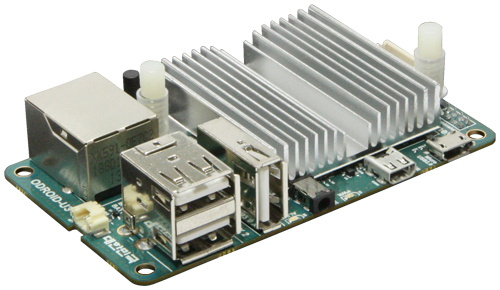
\includegraphics[width=0.45\columnwidth]{pictures/chapter3/odroid.jpg}
\caption{ODROID-U3}
\end{figure}

오픈소스 하드웨어 회사로 잘 알려진 국내 하드커널\footnote{\url{http://www.hardkernel.com/}}에서 개발한 오드로이드(ODROID-U3)는 ARM계열인 쿼드코어 1.7GHz Exynos 4412 Prime 를 사용하고 있어서 앞서 설명한 라즈베리파이 보다 월등한 성능 차이를 보이는 SBC의 한 종류이다. 더욱이 기본 OS로 루분투\footnote{\url{http://en.wikipedia.org/wiki/Lubuntu}}를 사용하고 있기에 우분투와 사용 방법은 비슷하면서도 LXDE\footnote{\url{http://ko.wikipedia.org/wiki/LXDE}} 데스크톱 환경을 사용하고 있어서 성능이 낮은 넷북, 휴대용 기기, 구형 PC에서도 매우 잘 돌아간다. 특히, 라즈베리파이에서는 영상 처리 혹은 Xtion, Kinect 같은 3차원 정보 취득에 있어서는 성능이 떨어지는 반면 오드로이드는 1.7GHz 쿼드코어와 2G RAM을 기본 탑재하고 있어서 사용함에 있어서 불편함이 없다.

오드로이드에 루분투를 설치하도록 하자. 오드로이드 우분투 자료실인 \url{http://odroid.in/ubuntu_14.04lts/} 에 접속하여 ubuntu-14.04.1lts-lubuntu-odroid-u-20141124.img.xz 을 다운로드 하자. 참고로 이 파일은 자주 갱신 되기 때문에 다운로드 받을시 언급한 버전이 아니더라도 ubuntu-14.04*으로 시작하는 가장 최신판을 다운로드 받으면 된다. 다운 받은 후 다음과 같이 압축을 해제하여 루분투의 ISO을 얻도록 하자.\\

\begin{lstlisting}[language=ROS]
$ xz -dv ubuntu-14.04.1lts-lubuntu-odroid-u-20141124.img.xz
\end{lstlisting}

압축 해제한 이미지 파일을 SD 카드에 넣도록 하자. 완전 포맷되지 않은 SD 카드의 경우, 기존 파티션을 삭제 하도록 하자. 파티션 수정을 위하여 GUI를 지원하는 disks를 이용할 것이다. 터미널 창에서 gnome-disks 를 실행하자. 그 뒤 디스크 목록에서 해당 SD 카드를 선택하면 기존에 사용했던 SD 카드라면 그림\ref{fig:partition_init2} 좌측과 같이 기존 파티션들이 보일 것이다. 그 하단의 \textbf{-} 버튼을 클릭하여 기존 파티션을 모두 삭제하여 모든 영역을 Free Space로 만들면 그림\ref{fig:partition_init2} 우측과 같은 결과를 얻을 수 있다.

\vspace{\baselineskip}
\begin{lstlisting}[language=ROS]
$ gnome-disks
\end{lstlisting}

\begin{figure}[h]
\centering
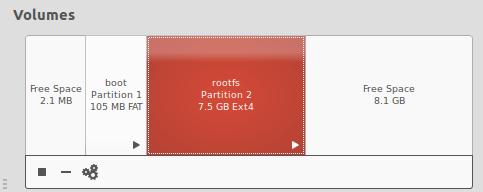
\includegraphics[width=0.49\columnwidth]{pictures/chapter3/odroid_partition1.png}
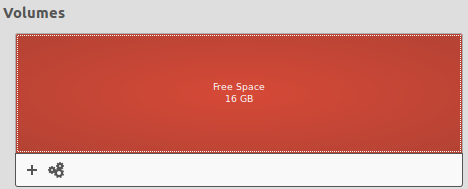
\includegraphics[width=0.48\columnwidth]{pictures/chapter3/odroid_partition2.png}
\caption{기존 파티션(좌)과 파티션 초기화(우)}
\label{fig:partition_init2}
\end{figure}

그 다음 그림\ref{fig:partition_restore} 좌측과 같이 disks 화면의 우측 상단의 버튼을 클릭하여 Restore disk image... 을 실행하자. 그림\ref{fig:partition_restore} 우측처럼 imgae to Restore 의 파일 선택에서 이전 압축 해제한 이미지 파일을 선택하고 Start Restoring 를 클릭하면 루분투 이미지가 리스토어 되게 된다. 리스토어가 완료되면 그림\ref{fig:lubuntu_partition_new} 과 같이 새로운 파티션들이 생성 되었음을 확인할 수 있다.

\begin{exercise}[SD 카드에 이미지 파일 넣는 다른 방법]
disks 이외에도 dd bs=4M if=ubuntu-14.04.1lts-lubuntu-odroid-u-20141124.img of=/dev/sdd 처럼 dd 명령어를 이용하는 방법이 있으며, 윈도우즈의 경우 Win32DiskImage\footnote{\url{http://sourceforge.net/projects/win32diskimager/}}를 이용하여 손쉽게 이미지 파이을 SD카드에 넣을 수 있다.
\end{exercise}

\begin{figure}[h]
\centering
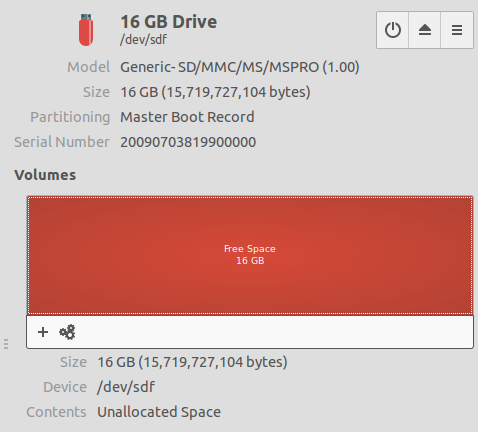
\includegraphics[width=0.49\columnwidth]{pictures/chapter3/odroid_sd.png}
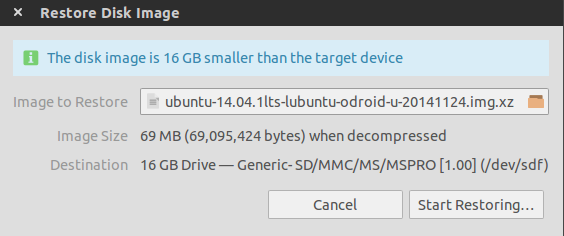
\includegraphics[width=0.49\columnwidth]{pictures/chapter3/odroid_restore.png}
\caption{디스크가 초기화된 상태(좌), 리스토어 준비 과정}
\label{fig:partition_restore}
\end{figure}


\begin{figure}[h]
\centering
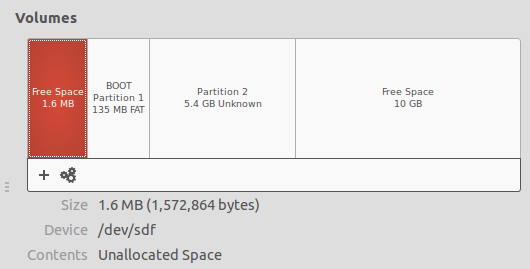
\includegraphics[width=0.6\columnwidth]{pictures/chapter3/odroid_partition3.png}
\caption{새롭게 구성된 파티션}
\label{fig:lubuntu_partition_new}
\end{figure}

리스토어한 SD 카드를 오드로이드에 삽입한 후, 전원을 넣고 부팅되면 그림\ref{fig:lxde}와 같이 루분투의 LXDE 데스크톱 환경을 볼 수 있다. 참고로 초기에는 로그인시 패스워드를 요구하지 않는다. 나중에 직접 패스워드를 지정해주도록 하자.

현재 SD 메모리의 일부 부분만 사용할 수 있도록 되어 있기 때문에 메모리를 리사이즈 할 필요가 있다. LXDE 화면 하단의 xterm 을 실행하여 다음과 같이 오드로이드 유틸리티를 실행하자. 그 후 그림\ref{fig:odroid_utility}와 같이 메모리 리사이즈를 하기 위하여 4.Resize your root partition 를 선택하여 리사이징을 해주자. 리사이징이 완료되었으며 아래와 같이 재부팅을 하자.

\begin{lstlisting}[language=ROS]
$ sudo odroid-utility.sh 
$ sudo reboot 
\end{lstlisting}

\begin{figure}[h]
\centering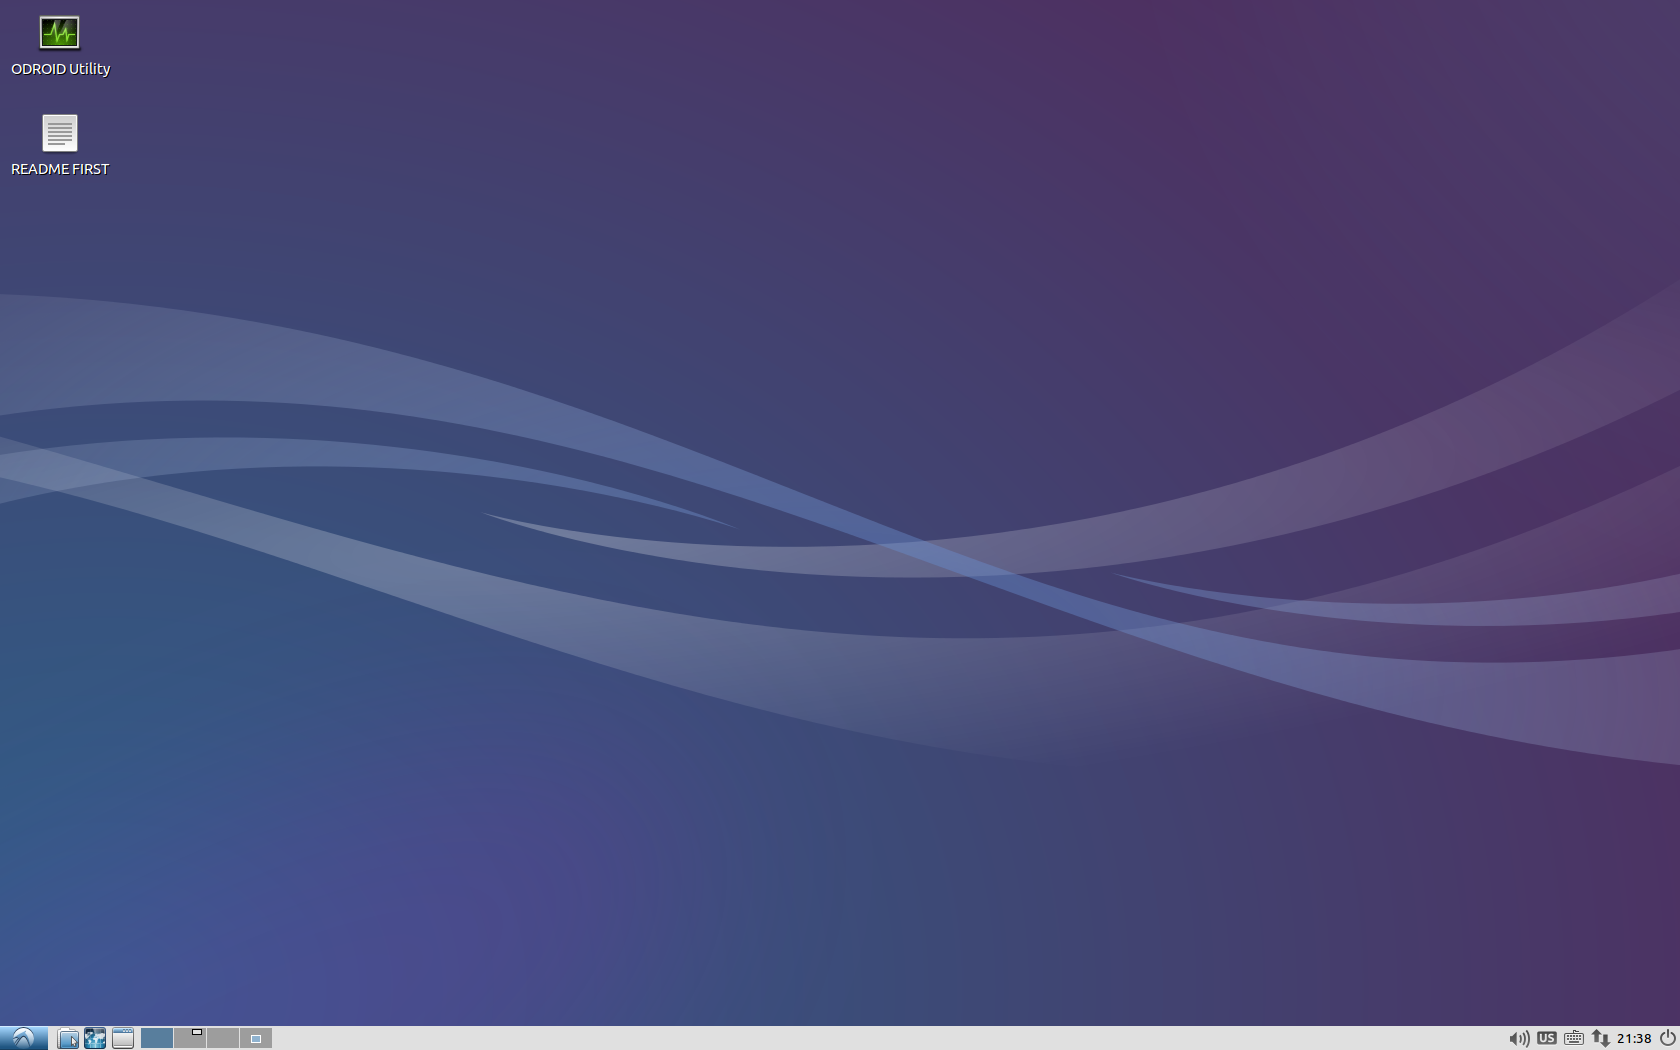
\includegraphics[width=0.7\columnwidth]{pictures/chapter3/odroid_LXDE.png}
\caption{LXDE 데스크톱}
\label{fig:lxde}
\end{figure}

\begin{figure}[h]
\centering
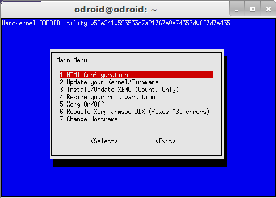
\includegraphics[width=0.49\columnwidth]{pictures/chapter3/odroid_option1.png}
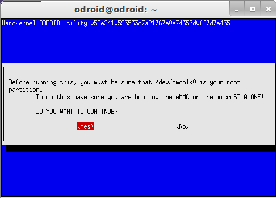
\includegraphics[width=0.49\columnwidth]{pictures/chapter3/odroid_option2.png}
\caption{오드로이드 유틸리티 화면과 리사이징 과정}
\label{fig:odroid_utility}
\end{figure}

\newpage

그 다음 다음의 명령어로 ROS Indigo를 설치하자.

\begin{lstlisting}[language=ROS]
$ sudo update-locale LANG=C LANGUAGE=C LC_ALL=C LC_MESSAGES=POSIX
$ sudo sh -c 'echo "deb http://packages.namniart.com/repos/ros trusty main" > /etc/apt/sources.list.d/ros-latest.list'
$ wget http://packages.namniart.com/repos/namniart.key -O - | sudo apt-key add -
$ sudo apt-get update
$ sudo apt-get install ros-indigo-ros-base
$ sudo apt-get install python-rosdep
$ sudo rosdep init
$ rosdep update
$ echo "source /opt/ros/indigo/setup.bash" >> ~/.bashrc
$ source ~/.bashrc
$ sudo apt-get install python-rosinstall
\end{lstlisting}

다음에는 다음과 같이 catkin work space 폴더를 만들고 catkin\_make 가 정상 작동하는지 살펴보자. 마지막으로 마지막으로 roscore 가 동작하는지 확인까지 마치면 모든 설치가 완료된 것이다. 추가적인 개발 환경 설정은 \textbf{섹션~\ref{subsec:envrionment}~\nameref{subsec:envrionment}(pp.\pageref{subsec:envrionment})}을 참고하도록 하자.

\begin{lstlisting}[language=ROS]
$ source /opt/ros/indigo/setup.bash
$ mkdir -p ~/catkin_ws/src
$ cd ~/catkin_ws/src
$ catkin_init_workspace
$ cd ~/catkin_ws/
$ catkin_make
$ roscore
\end{lstlisting}

\begin{figure}[h]
\centering
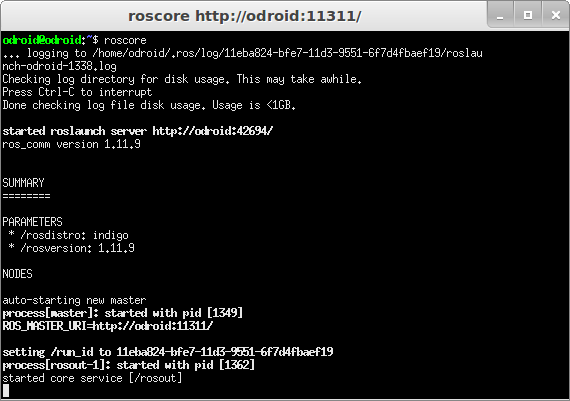
\includegraphics[width=0.7\columnwidth]{pictures/chapter3/odroid_roscore.png}
\caption{roscore 테스트}
\end{figure}

%-------------------------------------------------------------------------------


































































%-------------------------------------------------------------------------------